\section{Beamer-Beispiele}

\begin{frame}
\frametitle{Itemize und enumerate}
bullet points: itemize, Nummerierung: enumerate
\begin{itemize}
\item \textbf{EMMA} and \emph{motor modules}
\item Spreading activation with :bll 0.3 :mas 3 :rt 0 :ga 1
    :retrieval-activation 4 :visual-activation 2 :imaginal-activation 8
\item New TWM nodes created in imaginal buffer to keep parsing state
    and context in goal buffer
\item Word frequencies from dlexdb.de for base levels and EMMA
\end{itemize}
\end{frame}

\begin{frame}
\frametitle{Eine Tabelle}
\begin{table}[h]
\begin{center}
\begin{tabularx}{9cm}{Xll}
\toprule
Condition (2 items, 6 subjects) & DA & IA \\\midrule
Experiment (unreliable) & 3824ms & 3946ms \\
Model 1 & 3242ms & 3323ms \\
Model 2 & 3527ms & 3293ms \\
\bottomrule%
\end{tabularx}%
\end{center}%
\end{table}
\end{frame}

\begin{frame}[containsverbatim=true]
\frametitle{Quellcode anzeigen}
[containsverbatim=true] nach frame-Beginn nicht vergessen

\vskip 20pt

\begin{lstlisting}
for c in range(k):
   Mus[:,c]=X.T[np.where(rPrime==c)].T.mean(1)
\end{lstlisting}
\center{vs.}
\begin{lstlisting}
for i in range(k):
   mu[:,i] = np.mean(X[:,raux==i],axis=1)
\end{lstlisting}
\end{frame}

\begin{frame}[containsverbatim=true]
\frametitle{Grafiken einbinden}
Zur Skalierung einfach den Faktor ohne Multiplikationszeichen vor die
Breitenangabe schreiben.
\begin{figure}
\center{%
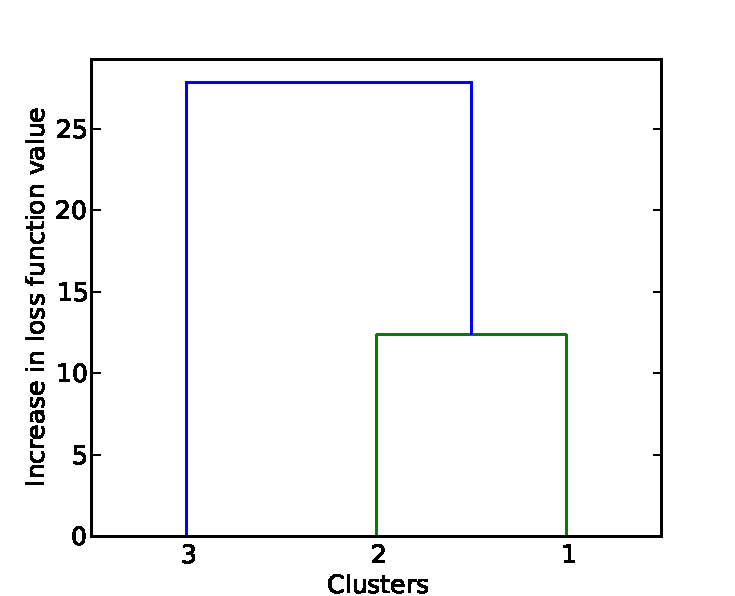
\includegraphics[width=.75\linewidth]{fig3}}
\end{figure}
\end{frame}